
Note to self: normalisation does not work for Q2Q1.

All the following benchmarks are isoviscous with $\eta=1$ and are valid in the unit square domain. 
As such the scaling coefficient between blocks $\K$ and $\G$ of the Stokes matrix (see Section~\ref{XYZ}) 
is 1 and won't play any role in the results. 

REDO all with aspect

According to Jenkins \etal (2014) \cite{jejl14}, Grad-div stabilization results from adding
$\vec{0} = - \gamma \vec\nabla (\vec\nabla\cdot \vec\upnu)$ to the continuous Stokes
equations, i.e.:
\[
-\nabla p  + \nabla \cdot ( 2 \eta \dot{\bm \varepsilon}) + \rho \vec{g} 
= - \gamma \vec\nabla (\vec\nabla\cdot \vec\upnu)
\]
We immediately notice that the aditional term is in fact identical to the penalty term and 
its weak form and discretisation is worked out in Section~\ref{XXX}, so that 
the matrix $\K$ then becomes:
\[
\K = \int {\bm B}^T \cdot [ \gamma {\bm K} + \eta {\bm C} ] \cdot {\bm B} \; dV
\]
with 
\[
{\bm C}=
\left(
\begin{array}{ccc}
2 & 0 & 0 \\
0 & 2 & 0 \\
0 & 0 & 1 
\end{array}
\right)
\qquad
{\bm K}=
\left(
\begin{array}{ccc}
1 & 1 & 0 \\
1 & 1 & 0 \\
0 & 0 & 0 
\end{array}
\right)
\]
The implementation is then trivial. Surprisingly in the papers on the grad-div stabilisation 
the penalty method is never mentioned (?) although John \etal state that 
"[...] it shall be emphasized that large
contributions of the grad-div stabilization result in linear systems of equations with
large condition numbers", which is a well know problem of the penalty method.

In this case $\gamma>0$ but another parallel can be drawn when $\gamma = -\frac{2}{3}\eta$. In that case
\[
 \nabla \cdot ( 2 \eta \dot{\bm \varepsilon}) + \gamma \vec\nabla (\vec\nabla\cdot \vec\upnu)
=
 \nabla \cdot ( 2 \eta \dot{\bm \varepsilon}) -\frac{2\eta}{3} \vec\nabla (\vec\nabla\cdot \vec\upnu)
=
 \nabla \cdot 2 \eta ( \dot{\bm \varepsilon} -\frac{1}{3} (\vec\nabla\cdot \vec\upnu) {\bm 1} )
= 
 \nabla \cdot 2 \eta \dot{\bm \varepsilon}^d 
\]
Obviously $\gamma$ should not be `too negative', otherwise terms on the diagonal 
of $\gamma {\bm K} + \eta {\bm C} $
will be negative and this will cause problems. 

In what follows I have implemented what I think the grad-div method is, with 
rather limited/puzzling (?) results.
Rather importantly John \etal conclude that ``the
grad-div stabilization might improve the pressure-robustness in certain situations but
it is not a remedy''. 

\Literature: \cite{ollh09}

%---------------------------------------------------------------------
\subsubsection*{Experiment=1: Donea \& Huerta manufactured solution}

I carry out this benchmark to make sure that the code behaves as expected and that the
error rates are what we expect: 3rd order for velocity, second order for pressure 
for both $Q_2\times Q_1$ and $Q_2\times P_{-1}$ elements (see for instance 
Thieulot \& Bangerth \cite{thba22}).

\begin{center}
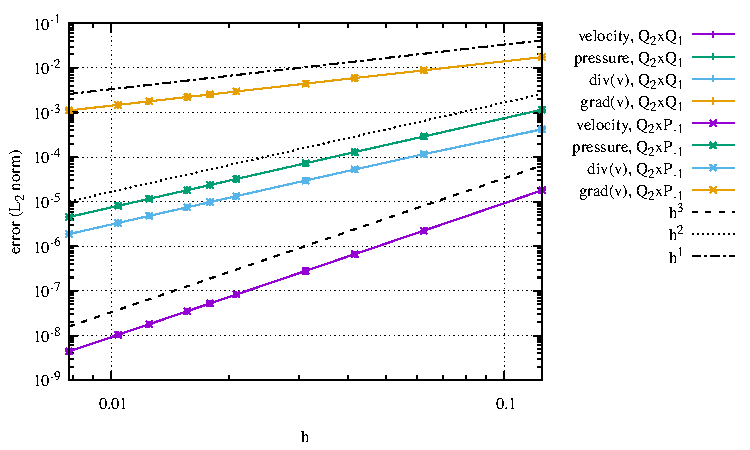
\includegraphics[width=8cm]{python_codes/fieldstone_104/results/exp1/errors.pdf}
\end{center}


%---------------------------------------------------------------------
\subsubsection*{Experiment=2: example 1.1 in John \etal (2017)}
Following John \etal (2017) \cite{jolm17} we 
postulate the following velocity and pressure fields:
\begin{eqnarray}
\vec{\upnu}(x,y) &=& \vec{0} \nn\\
p(x,y) &=& \Ranb ( y^3-y^2/2+y-7/12 ) \nn
\end{eqnarray}
with $\eta=1$ and the buoyancy force vector is
\[
\vec{b}=
\left(
\begin{array}{c}
0 \\ \Ranb(1-y+3y^2)
\end{array}
\right)
\]

\begin{center}
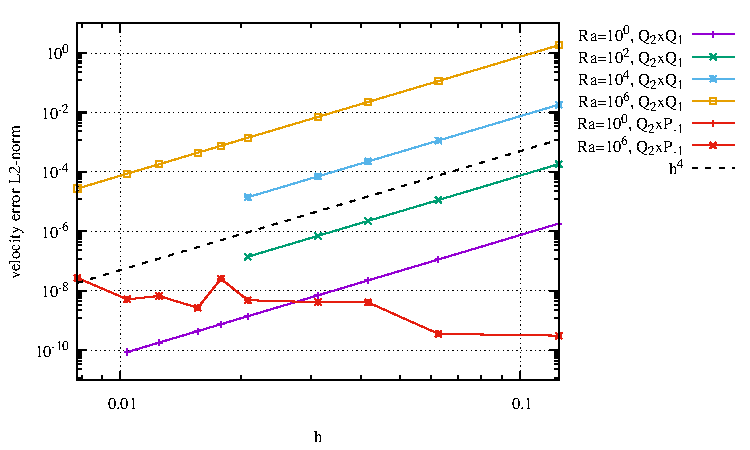
\includegraphics[height=4cm]{python_codes/fieldstone_104/results/exp2/errors.pdf}
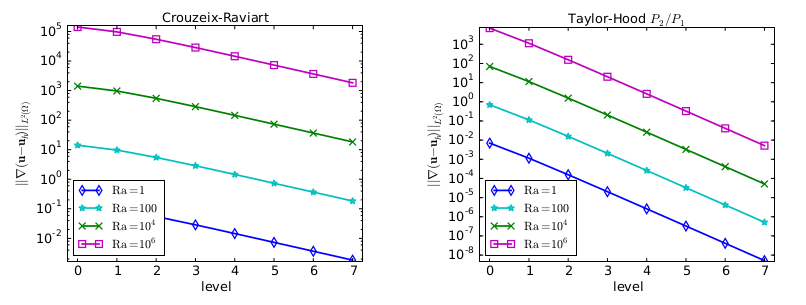
\includegraphics[height=4cm]{python_codes/fieldstone_104/results/exp2/jolm17a}\\
{\captionfont Left: this stone; Right: taken from \cite{jolm17}}
\end{center}

We find that the velocity error magnitude for the $Q_2\times Q_1$ element
scales with the Rayleigh number, and 
more surprisingly (?) that its convergence is quartic.
However, the velocity error magnitude for the $Q_2\times P_{-1}$ 
remains very low independently of the Rayleigh number

\begin{center}
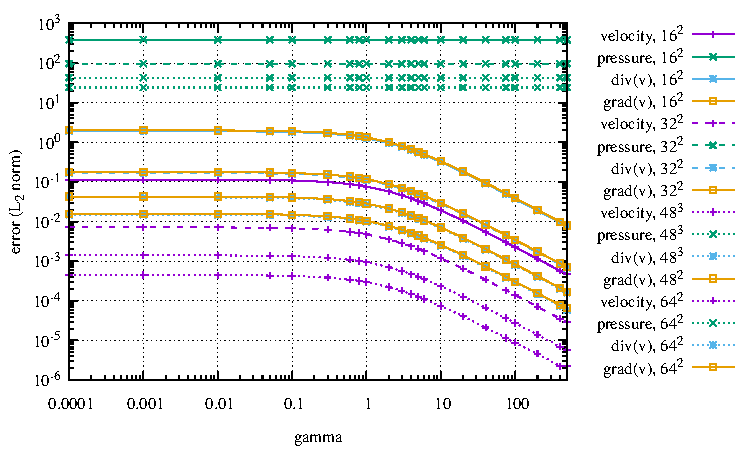
\includegraphics[height=6cm]{python_codes/fieldstone_104/results/exp2/gamma/errors.pdf}
\end{center}

%---------------------------------------------------------------------
\subsubsection*{Experiment=3,4,5: }

These three manufactured solutions come from Jenkins \etal (2014) \cite{jejl14}.
The velocity is the same in all cases, $\vec{\upnu}=(\cos 2\pi y , \sin 2\pi x)$
while the three pressure fields are
\begin{eqnarray}
p_1(x,y) &=& \sin (2\pi y)  \nn\\
p_2(x,y) &=& \sin (8 \pi y)   \nn\\
p_3(x,y) &=& 10^4 \sin (2\pi y) \nn
\end{eqnarray}
We need to compute the vector $\vec{b}$ from these. 
The strain rate tensor is then 
\[
\dot{\bm \varepsilon}(\vec{\upnu}) = 
\left(
\begin{array}{cc}
0 &  - \pi \sin 2\pi y + \pi \cos 2 \pi x  \\
 - \pi \sin 2\pi y + \pi \cos 2 \pi x   & 0
\end{array}
\right)
\]
and then the full stress tensor:
\[
{\bm \sigma} = 
- p {\bm 1}+ 2 \eta \dot{\bm \varepsilon}
= \left(
\begin{array}{cc}
-p &  -2 \pi \eta (\sin 2\pi y -  \cos 2 \pi x)  \\
-2 \pi \eta (\sin 2\pi y -  \cos 2 \pi x)   & -p
\end{array}
\right)
\]
Finally
\[
-\vec{b} = 
\vec\nabla \cdot {\bm \sigma} = 
\left(
\begin{array}{c}
-\partial_x p - 4 \pi^2 \eta \cos 2\pi y  \\ 
-\partial_y p - 4 \pi^2 \eta \sin 2\pi x 
\end{array}
\right)
\]
We see that we have $\partial_x p_{1,2,3} =0$ so 
\[
\vec{b}
=
\left(
\begin{array}{c}
 4 \pi^2 \eta \cos 2\pi y  \\ 
\partial_y p + 4 \pi^2 \eta \sin 2\pi x 
\end{array}
\right)
\]

\begin{center}
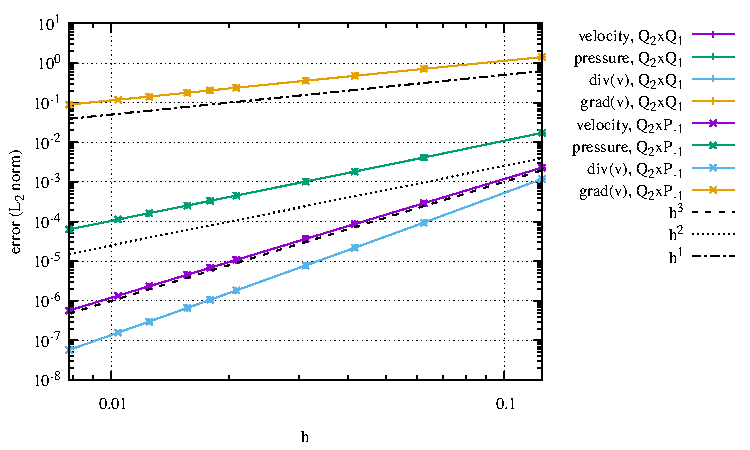
\includegraphics[width=5cm]{python_codes/fieldstone_104/results/exp3/errors.pdf}
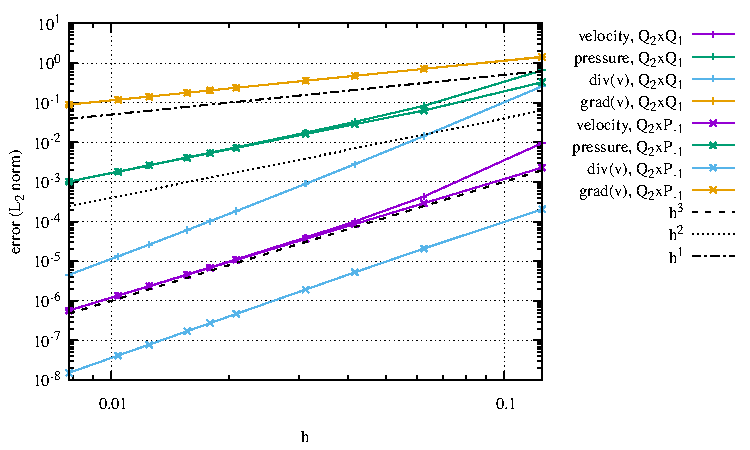
\includegraphics[width=5cm]{python_codes/fieldstone_104/results/exp4/errors.pdf}
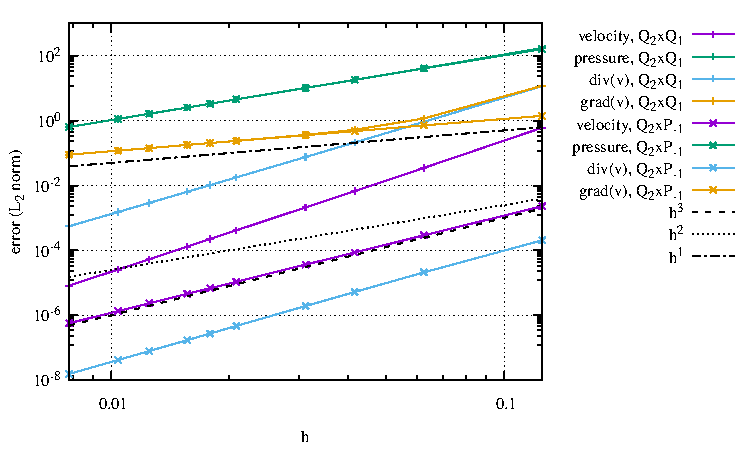
\includegraphics[width=5cm]{python_codes/fieldstone_104/results/exp5/errors.pdf}
\end{center}

We see that the Q2Q1 velocity error is much larger than the Q2P1 error in benchmark 3 
but that it converges again in a quartic manner.
Pressure errors are however identical.

%------------------------------------------------------------------------------------------
\subsubsection*{Experiment=6: manufactured solution in John \etal (2017) \cite{jolm17}}

See Section~\ref{ss:mmsjolm17} for details.

\begin{center}
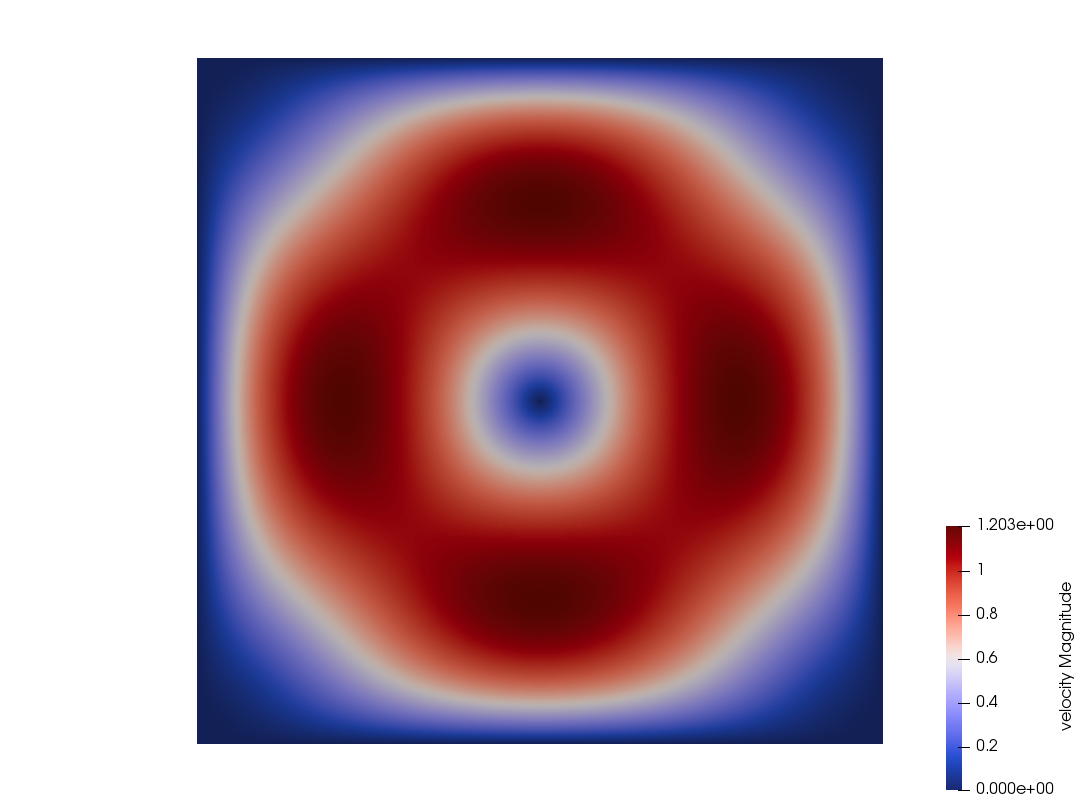
\includegraphics[width=5cm]{python_codes/fieldstone_104/results/exp6/vel}
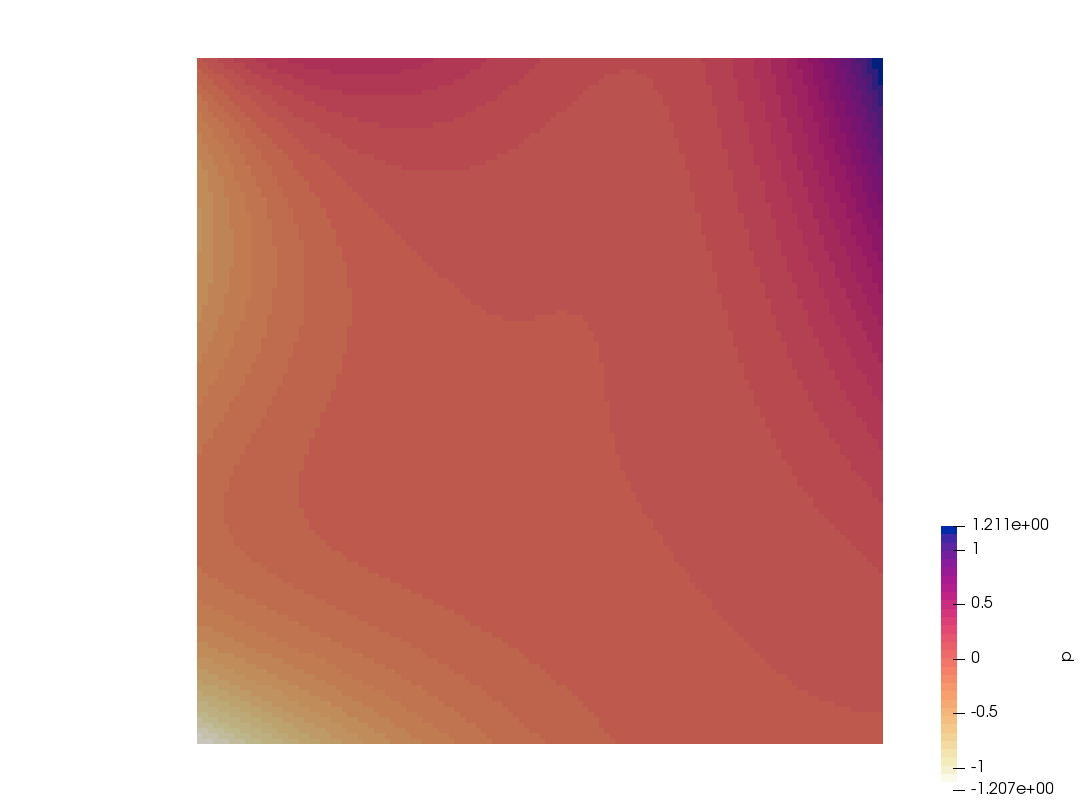
\includegraphics[width=5cm]{python_codes/fieldstone_104/results/exp6/press}
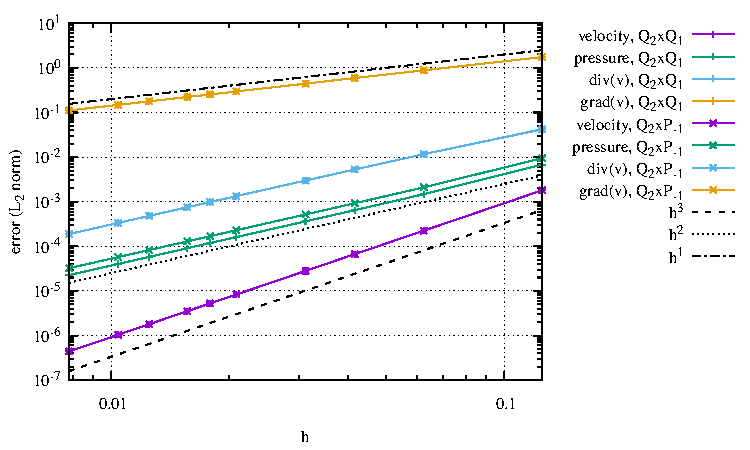
\includegraphics[width=5cm]{python_codes/fieldstone_104/results/exp6/errors.pdf}
\end{center}


\begin{center}
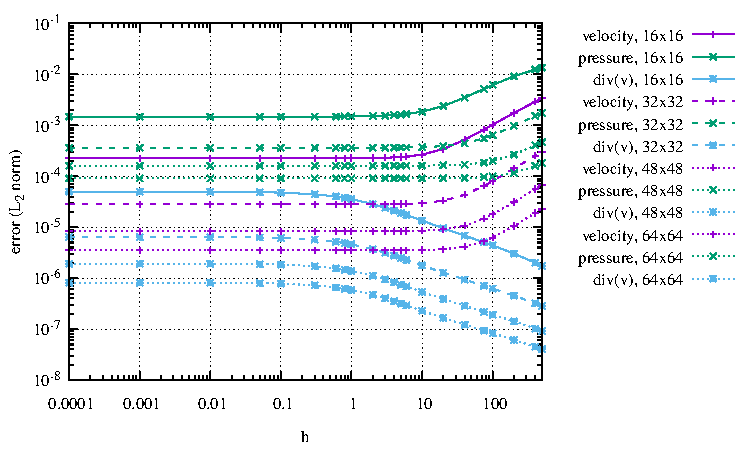
\includegraphics[height=6cm]{python_codes/fieldstone_104/results/exp6/gamma/errors.pdf}\\
{\captionfont errors as a function of $\gamma$.}
\end{center}



